\documentclass[12pt]{article}

\usepackage{amsmath}
\usepackage{amsthm}
\usepackage{tikz}

\title{EECS 440 HW6}
\author{Andrew Mason}

\begin{document}
\maketitle

\begin{enumerate}
  \item
    % 1
  \item
    % 2
    \begin{proof} A neural network with a single hidden layer and a single
      output unit all with sigmoid activation is equivalent to a network where
      the hidden unit activations are $\tanh$ functions, and the ouput unit
      still has a sigmoid activation.\\

      \begin{equation}
        \begin{split}
          \tanh(w,x,a,b)&=a\frac{e^{b\boldsymbol{w}\cdot \boldsymbol{x}}-
                                 e^{-b\boldsymbol{w}\cdot\boldsymbol{x}}}
                                {e^{b\boldsymbol{w}\cdot\boldsymbol{x}}+
                                 e^{-b\boldsymbol{w}\cdot\boldsymbol{x}}}\\
          &=a\frac{\frac{e^{2b\boldsymbol{w}\cdot \boldsymbol{x}}-1}
                   {e^{b\boldsymbol{w}\cdot\boldsymbol{x}}}}
                  {\frac{e^{2b\boldsymbol{w}\cdot\boldsymbol{x}}+1}
                   {e^{b\boldsymbol{w}\cdot\boldsymbol{x}}}}\\
          &=a\frac{e^{2b\boldsymbol{w}\cdot \boldsymbol{x}}-1}
                  {e^{2b\boldsymbol{w}\cdot\boldsymbol{x}}+1}\\
          &=a\left(1-\frac{2}
                         {e^{2b\boldsymbol{w}\cdot\boldsymbol{x}}+1}\right)\\
          \tanh(w,x,-2,-\frac{1}{2})&=
            \frac{2}
                 {e^{-\boldsymbol{w}\cdot\boldsymbol{x}}+1}-1\\
        \end{split}
      \end{equation}

      This expression is $2\times\text{sigmoid}(w,x)-1$. Which means the range
      of the function is (-1,1), whereas the range of the sigmoid function is
      (0,1). At this point, all we need is a function which maps from the range
      (-1,1) to the range (0,1); this defines the weights needed for the output
      unit. This is easy to do, since we can just map the values below zero to
      the range (0, 0.5), and the values $\geq0$ to the range
      $\left[0.5, 1\right)$, using the function $f(x)=\frac{x+1}{2}$.\\
    \end{proof}
  \item
    % 3
    We need an output layer that fires whenever $-7\leq x_1+x_2\leq7$.\\
    \begin{center}
      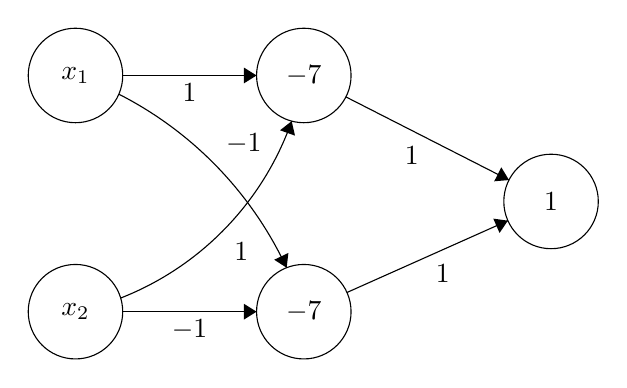
\begin{tikzpicture}[scale=0.2]
      \tikzstyle{every node}+=[inner sep=0pt]
      \draw [black] (13,-10.7) circle (3);
      \draw (13,-10.7) node {$x_1$};
      \draw [black] (13,-25.7) circle (3);
      \draw (13,-25.7) node {$x_2$};
      \draw [black] (27.5,-10.7) circle (3);
      \draw (27.5,-10.7) node {$-7$};
      \draw [black] (27.5,-25.7) circle (3);
      \draw (27.5,-25.7) node {$-7$};
      \draw [black] (43.2,-18.7) circle (3);
      \draw (43.2,-18.7) node {$1$};
      \draw [black] (16,-10.7) -- (24.5,-10.7);
      \fill [black] (24.5,-10.7) -- (23.7,-10.2) -- (23.7,-11.2);
      \draw (20.25,-11.2) node [below] {$1$};
      \draw [black] (26.731,-13.597) arc (-19.44059:-68.61736:18.78);
      \fill [black] (26.73,-13.6) -- (25.99,-14.18) -- (26.94,-14.52);
      \draw (23.05,-21.87) node [right] {$1$};
      \draw [black] (15.753,-11.887) arc (63.02359:25.03436:23.548);
      \fill [black] (26.41,-22.91) -- (26.52,-21.97) -- (25.62,-22.4);
      \draw (22.53,-15.04) node [right] {$-1$};
      \draw [black] (16,-25.7) -- (24.5,-25.7);
      \fill [black] (24.5,-25.7) -- (23.7,-25.2) -- (23.7,-26.2);
      \draw (20.25,-26.2) node [below] {$-1$};
      \draw [black] (30.17,-12.06) -- (40.53,-17.34);
      \fill [black] (40.53,-17.34) -- (40.04,-16.53) -- (39.59,-17.42);
      \draw (34.36,-15.2) node [below] {$1$};
      \draw [black] (30.24,-24.48) -- (40.46,-19.92);
      \fill [black] (40.46,-19.92) -- (39.53,-19.79) -- (39.93,-20.7);
      \draw (36.33,-22.71) node [below] {$1$};
      \end{tikzpicture}
    \end{center}
    Let the upper hidden layer node be $h_1$, the lower hidden layer node be
    $h_2$, and the output node be $y$. Now let`s trace the examples.\\
    \begin{enumerate}
      \item $x_1,x_2,y=-4,-4,-1$\\
        \begin{equation}
          \begin{split}
            h_1&=sign(-8+7)=-1\\
            h_2&=sign(8+7)=1\\
            y&=sign(0-1)=-1\\
          \end{split}
        \end{equation}
      \item $x_1,x_2,y=-1,-1,1$\\
        \begin{equation}
          \begin{split}
            h_1&=sign(-2+7)=1\\
            h_2&=sign(2+7)=1\\
            y&=sign(2-1)=1\\
          \end{split}
        \end{equation}
      \item $x_1,x_2,y=1,1,1$\\
        \begin{equation}
          \begin{split}
            h_1&=sign(2+7)=1\\
            h_2&=sign(-2+7)=1\\
            y&=sign(2-1)=1\\
          \end{split}
        \end{equation}
      \item $x_1,x_2,y=4,4,-1$\\
        \begin{equation}
          \begin{split}
            h_1&=sign(8+7)=1\\
            h_2&=sign(-8+7)=-1\\
            y&=sign(0-1)=-1\\
          \end{split}
        \end{equation}
    \end{enumerate}
  \item
    % 4
  \item
    % 5
\end{enumerate}
\end{document}
